

\documentclass[aspectratio=169]{beamer}
\usetheme{Madrid}
\usepackage[T2A]{fontenc}
\usepackage[utf8]{inputenc}
\usefonttheme{serif}



\usepackage{array}
\usepackage{colortbl}
\usepackage{hhline}
\usepackage[english,ukrainian,russian]{babel}
%\usepackage{fourier}
\usepackage{lmodern}


\usepackage{ textcomp }
\usepackage{ eqnarray }
\usepackage{ txfonts }
\usepackage{hyperref}
\DeclareUnicodeCharacter{00A0}{ }

\title{Відповіді на питання у форматі презентації}
 \logo{
   	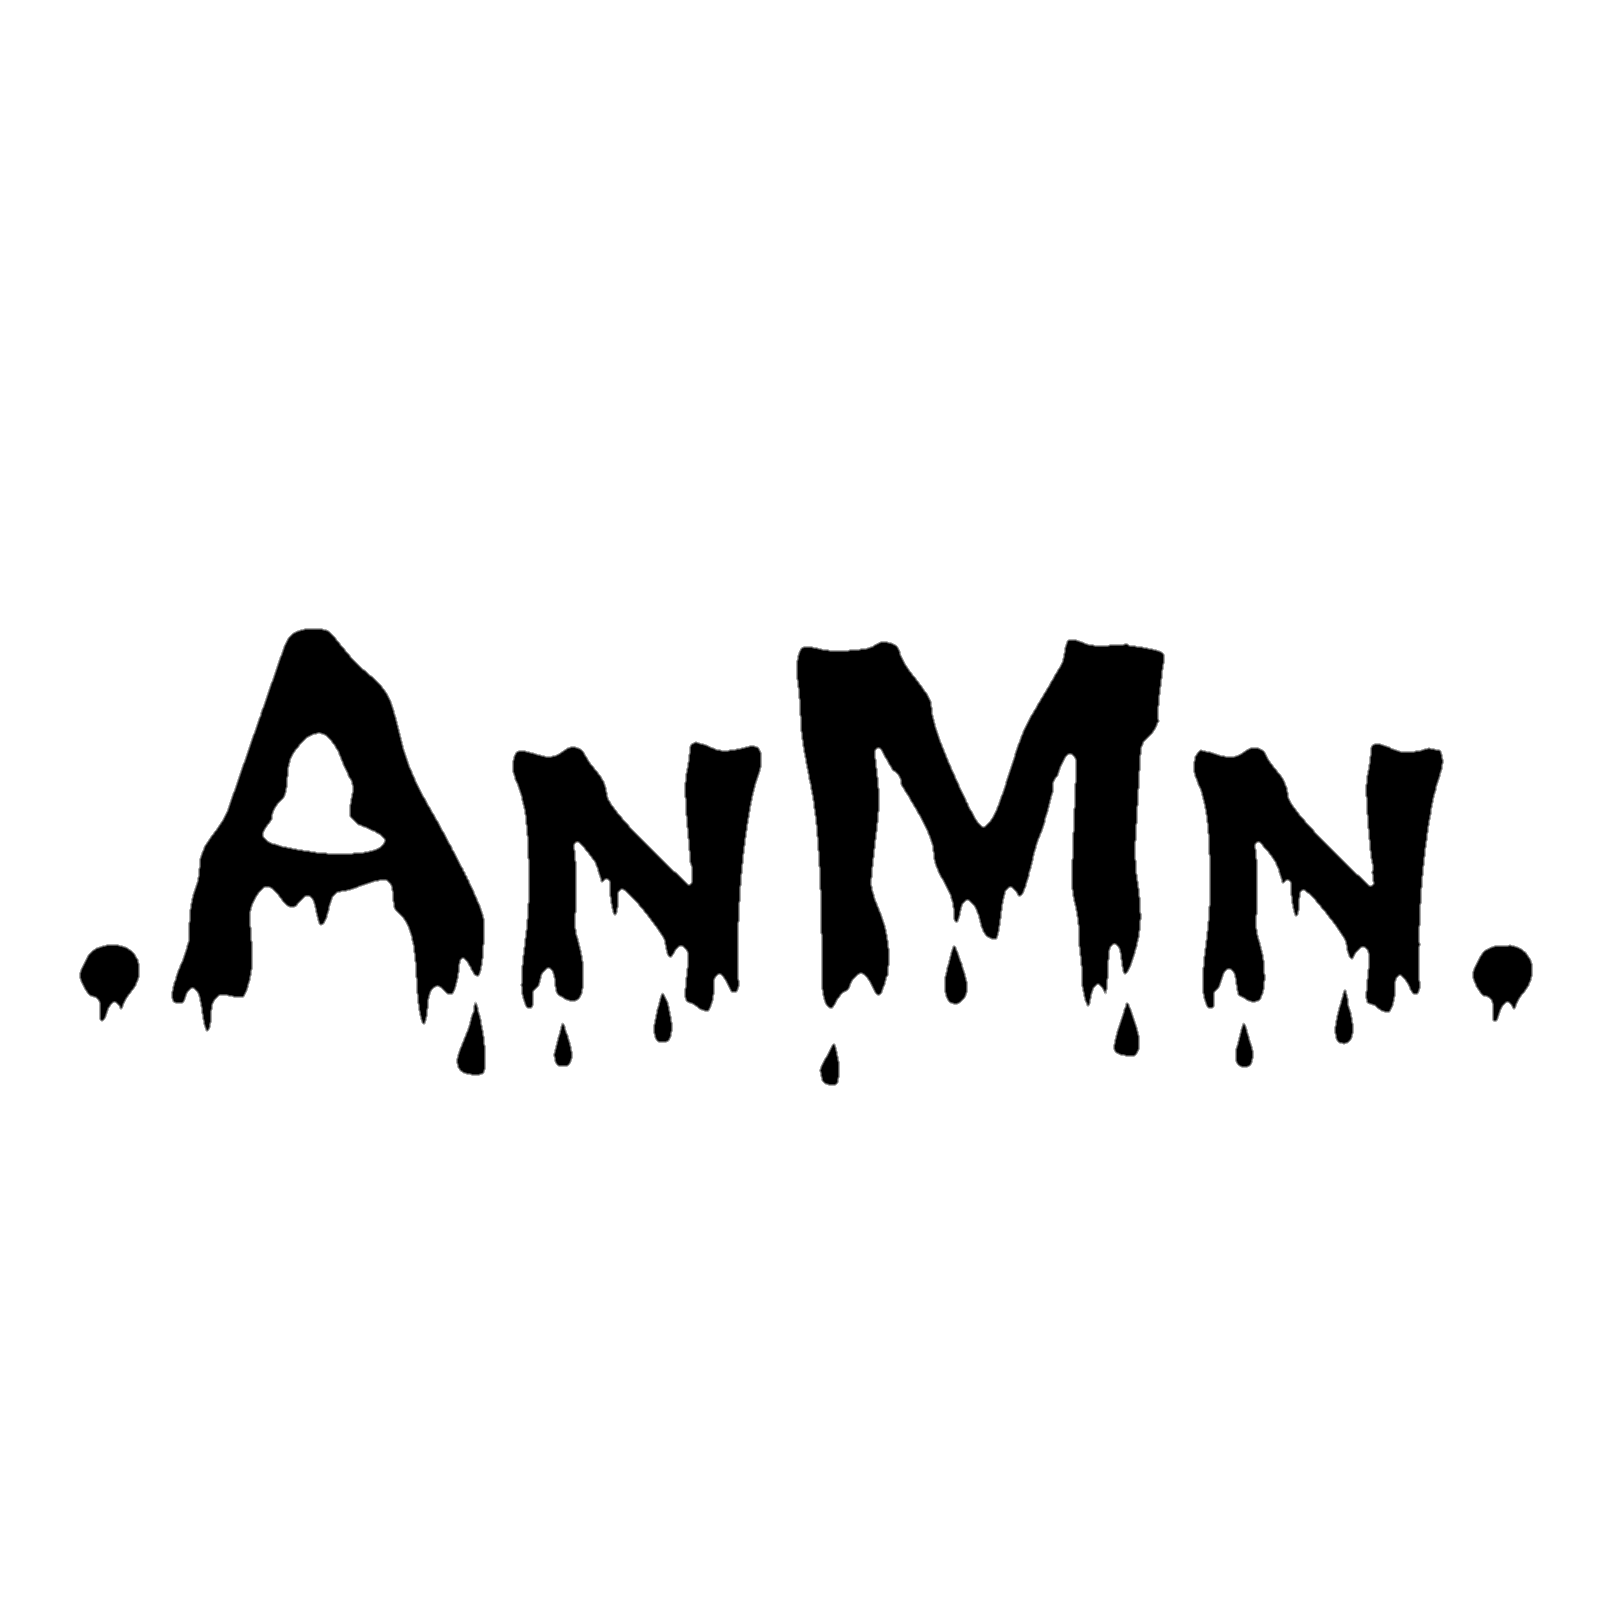
\includegraphics[width=1.5cm]{1590609722363.png}
   	\hspace{-1.1cm}
  	 } 
\author{Мнацаканов Антон}
\institute[] % (optional)
{
 \normalsize Faculty of Electronics\\
 group ДП-82\\
National Technical University of Ukraine "Igor Sikorsky Kyiv Polytechnic Institute" 
}
\begin{document}% начало презентации
\begin{frame}% первый слайд
\titlepage{}
\end{frame}



{

\begin{frame}% второй слайд
	
		\large\textcolor{blue}{\textbf{Питання №1:}}
		\\Назвіть основні стандартні технологічні процеси виготовлення  електронних і механічних компонентів та вузлів \textbf{\underline{мікросистемної}} техніки. 
		   Назвіть основні специфічні технологічні процеси.
\end{frame}
}



{
\title{\textcolor{orange}{Головні визначення}}
\usebackgroundtemplate{ 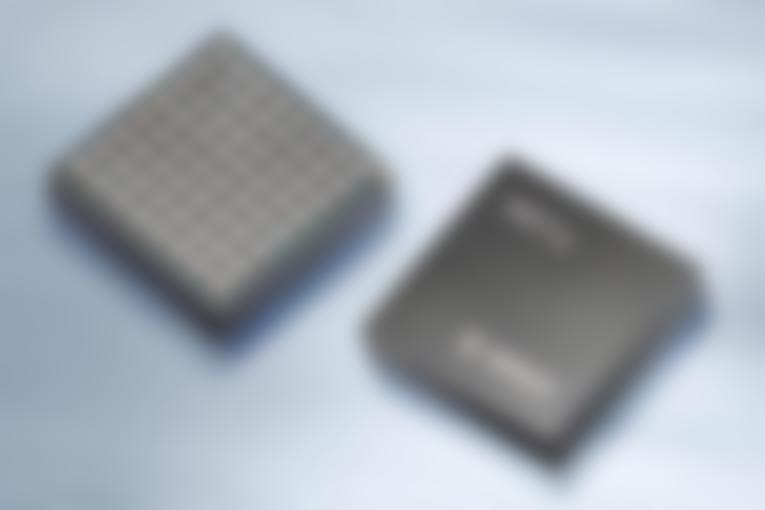
\includegraphics[width=\paperwidth]{s.jpg} }
\begin{frame}
\center{\fcolorbox{red}{yellow}{А щож таке мікросистема та технологія її виготовлення?}}\\

\textbf
	 {
	  \large Це інтегрована інформаційно-керуюча система, функціонально і структурно об'єднана для збору і обробки інформації в 
          реальному масштабі часу і подальшого вироблення впливів на виконавчі елементи або об'єкт управління.\\
          Мікросистемна технологія: послідовність технологічних операцій групової мікрообробки поверхні матеріалу заготовки з метою виготовлення, складання, корпусування і 
          вимірювання елементів, компонентів і вузлів мікросистеми.
          }
\end{frame}
}



{
\title{\textcolor{orange}{Основні види технології}}
\usebackgroundtemplate{ 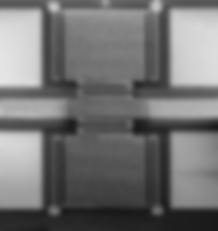
\includegraphics[width=\paperwidth]{f.jpg} }
\begin{frame}
\center{\fcolorbox{black}{green}{Базові технології мікро- і наносистемної техніки}}\\
\setlength\arrayrulewidth{2pt}\arrayrulecolor{blue}
\setlength\doublerulesep{2pt}\doublerulesepcolor{yellow}
\begin {center}
\begin{tabular}{||c||c||c||c||}
\hhline{|t:=:t:=:t:=t:=:t|}
\textcolor{orange}{EFAB} & \textcolor{green}{LIGA}& \textcolor{cyan}{SUMMiT} & \textcolor{magenta}{МUMPs}\\
\hhline{|b:=:b:=:b:=b:=:b|}
\end{tabular}
\end{center}
\end{frame}
}



{
\title{\textcolor{orange}{EFAB та LIGA}}
\usebackgroundtemplate{ 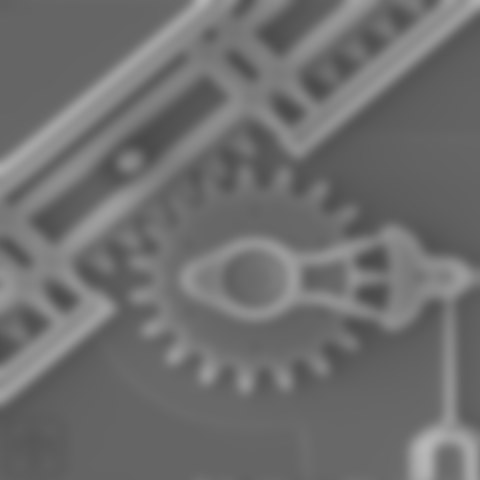
\includegraphics[width=\paperwidth]{w.jpg} }
\begin{frame}
\begin{flushleft}
\textcolor{orange}{\textbf\large 1.EFAB }
	(абревіатура від слів Electrochemical FABrication)-технологія. Вона грунтується на гальванічному осадженні металів на ізолюючі поверхні, з подальшим травленням структур в 		ізоляційному матеріалі, що дозволяє створювати, в тому числі тривимірні мікроструктури. Основними розробниками цієї технології є Information Science Institute (ISI) та University of 	Southem Calofornia. EFAB –технологія не вимагає надчистих приміщень, повністю автоматизована та має меншу кількість технологічних етапів.\\
\textcolor{green}{\textbf\large2.LIGA }
	(абревіатура від слів Litographie – літографія та Galvanoformung- гальванообробка) - техгологія. Ця об’ємна технологія і розроблена фахівцями німецького Центру ядерних 			досліджень (Карлсруе) з використанням жорсткого випромінювання синхротрона, прецезійного лиття полімерів заданої форми та гальванічного осадження металів на 			мікроповерхнях.Випромінювання синхротрона має малу кутову розбіжність і спроможне проникати в глибину полімеру на декілька міліметрів, що дозволило створювати об’ємні 		структури.
\end{flushleft}
\end{frame}
}



{
\title{\textcolor{orange}{SUMMiT та МUMPs}}
\usebackgroundtemplate{ 
\includegraphics[width=\paperwidth]{2.jpg} }
\begin{frame}
\begin{flushleft}
\textcolor{cyan}{\textbf\large 3.SUMMiT} 
	(абревіатура від слів Sandia Ultra-planar Multi-level MEMS Technology)-технологія. Це поверхнева технологія виготовлення (М,Н,О)ЕМС і ґрунтується на формуванні чотирьохшарової 	полікристалічної кремнієвої механічної структури, де перший нерухомий шар (кремнієва підкладка) утворює механічну і електричну основу для решта трьох рухомих шарів. SUMMiT 	технолгія легко інтегрується в кремнієву ІС. Механічні структури МЕМС систем створюються методами тонкоплівкової фотолітографії та хімічного травлення. Розроблена 			п’ятишарова SUMMiT-V технологія, спроможна створювати 24-битні механооптичні замки.\\
\textcolor{magenta}{\textbf\large4.МUMPs} 
	(Multi User MEMS Process) –технологія. Це тришарова поверхнева технологія полікремнієвого процесу виготовлення МЕМС. Вона складається із створення ізоляційного шару
	 $\mathrm{Si_3 N_4}$, шару полікремнію, на
	поверхні якого формуються рухомі частини із двох інших структурних шарів полікремнію. За потреби наносяться шари для виготовлення масок фотолітографії для створення 		сенсорів і актюаторних елементів та шар металізації. Недоліком цього процесу\\ є неможливість виготовлення елементів МЕМС із іншого матеріалу окрім полікремнію.
\end{flushleft}
\end{frame}
}



{
\title{\textcolor{red}{\fcolorbox{black}{green}{\large EFAB}}}
\usebackgroundtemplate{ 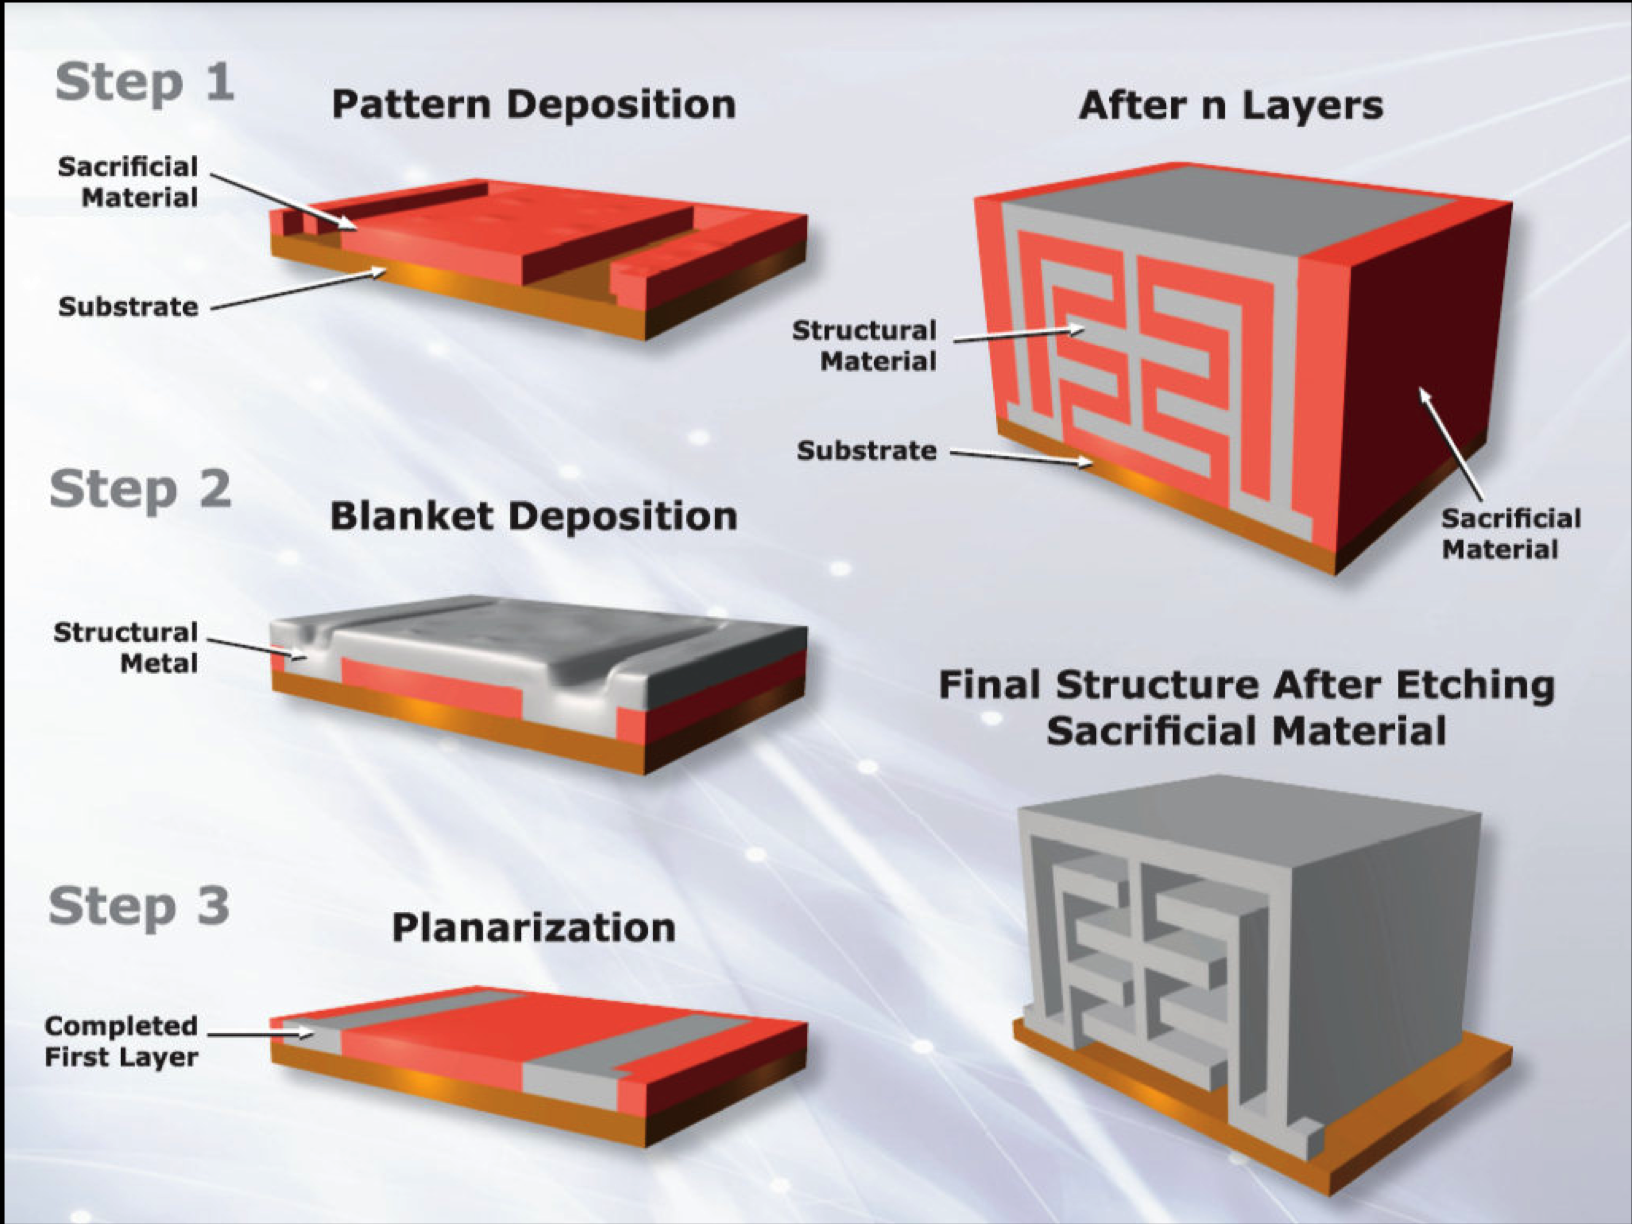
\includegraphics[width=\paperwidth,height=9cm]{a.png} }
\begin{frame}
\end{frame}
}



{
\title{}
\usebackgroundtemplate{ 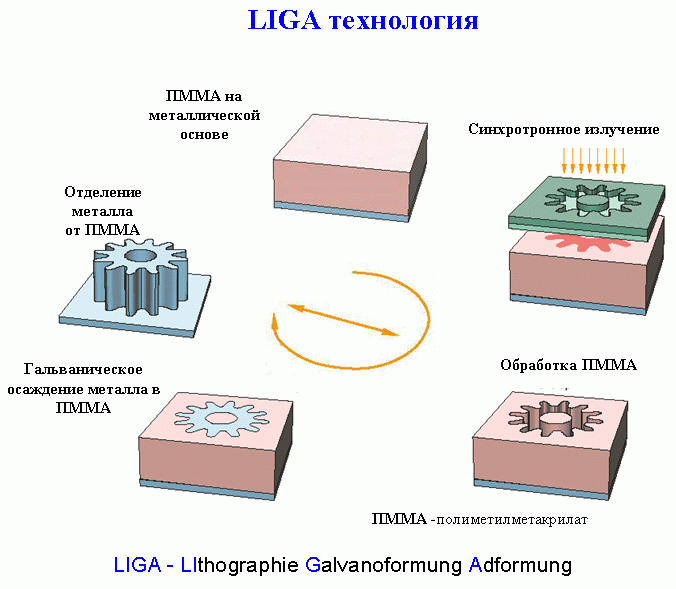
\includegraphics[width=\paperwidth,height=8.7cm]{liga.jpg} }
\begin{frame}
\end{frame}
}



{
\title{}
\usebackgroundtemplate{ 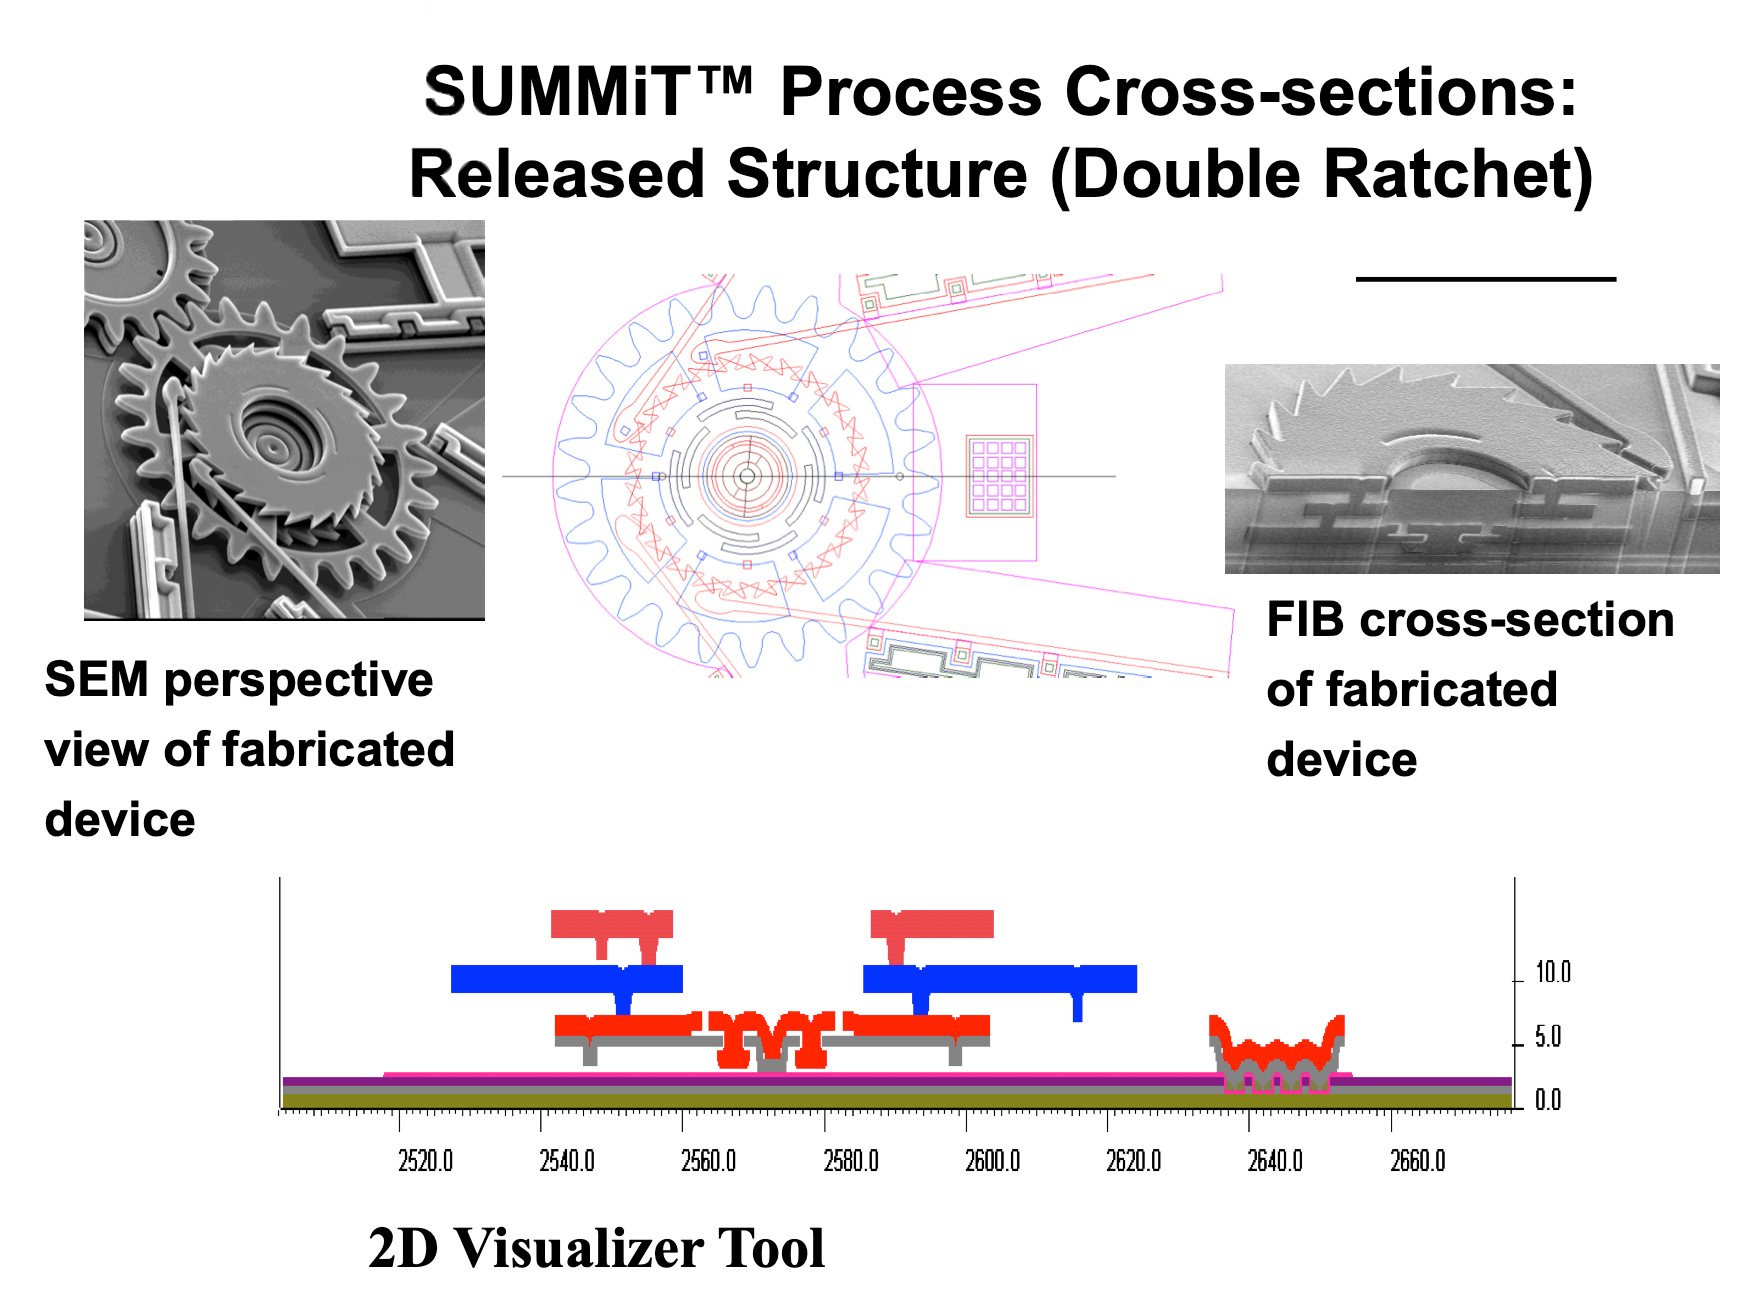
\includegraphics[width=\paperwidth,height=8.7cm]{summit1.jpg} }
\begin{frame}
\end{frame}
}



{
\title{}
\usebackgroundtemplate{ 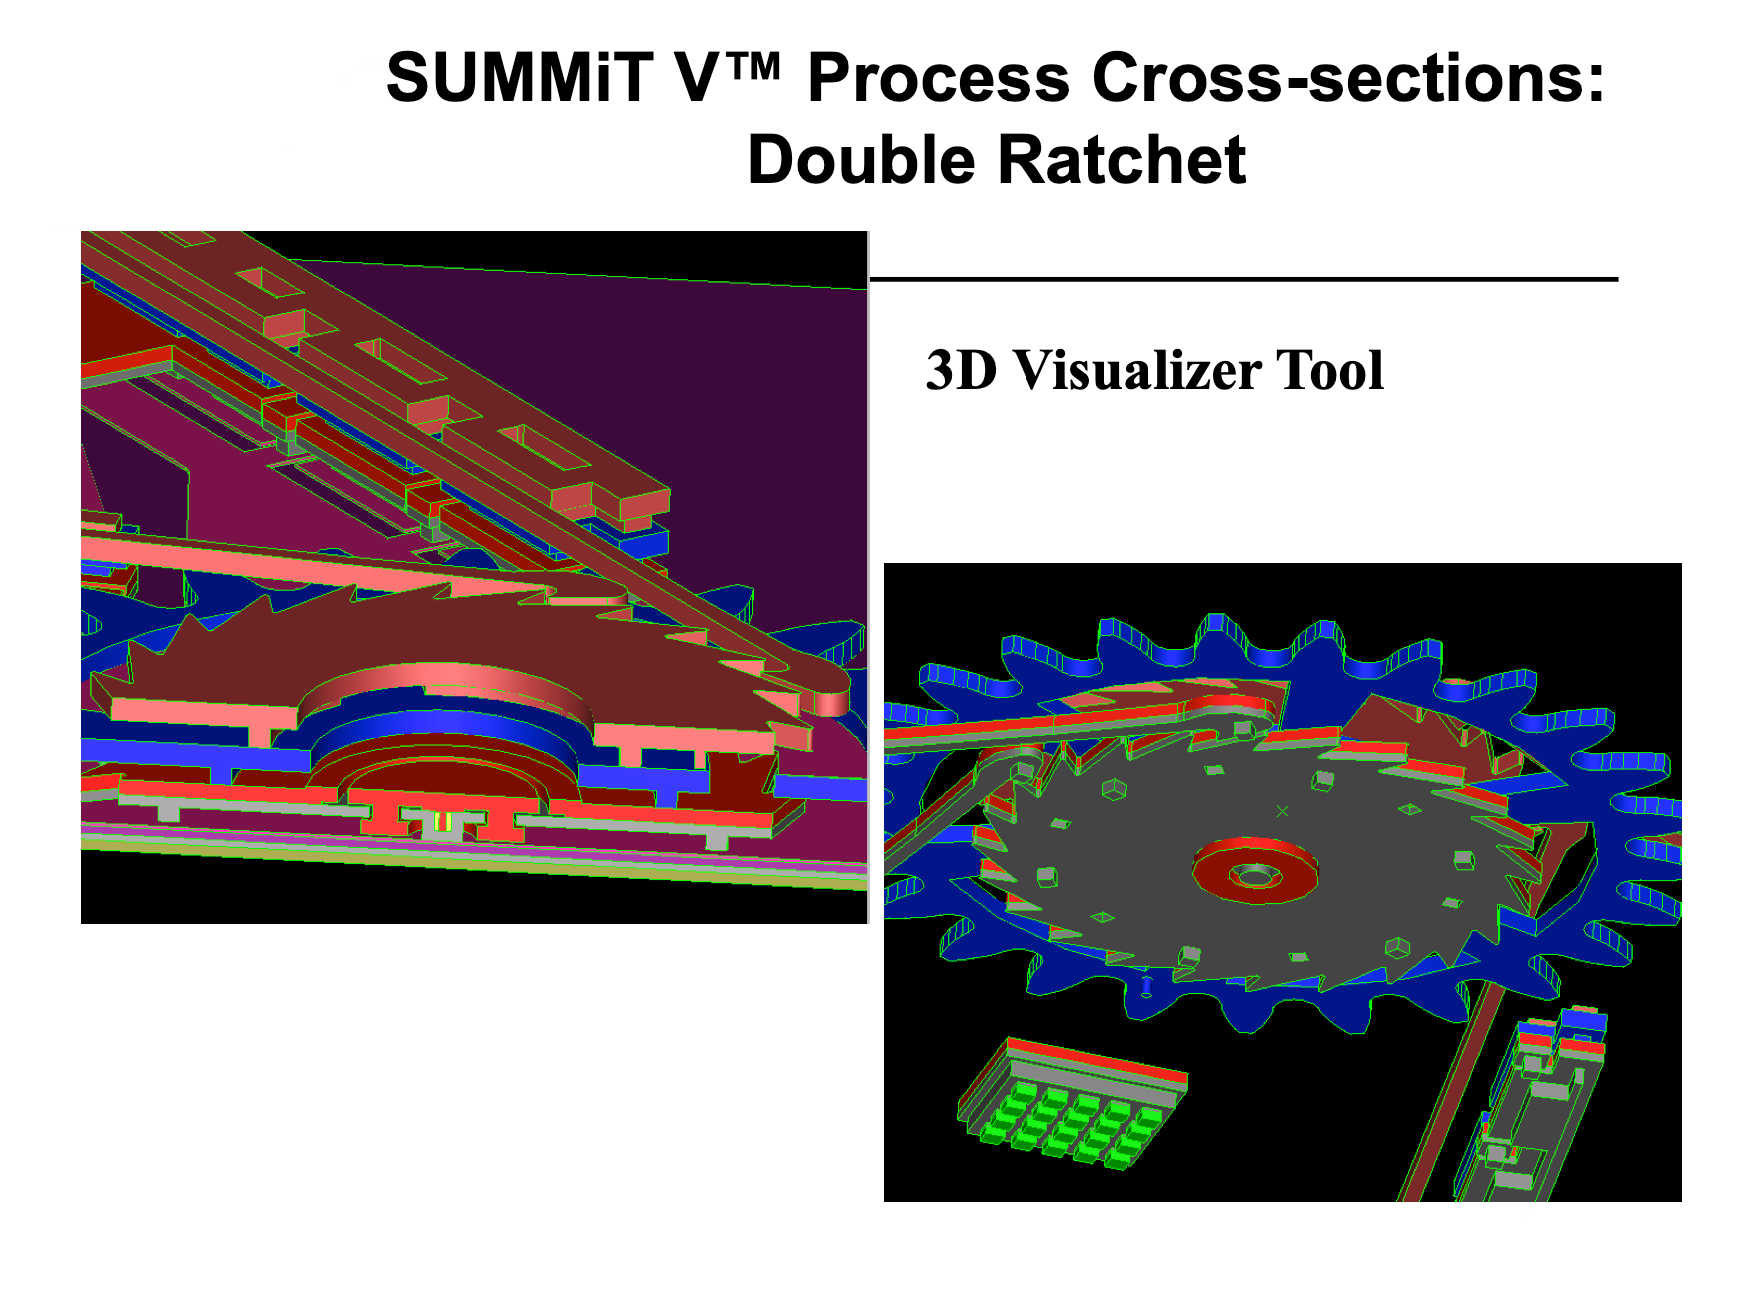
\includegraphics[width=\paperwidth,height=8.7cm]{summit2.jpg} }
\begin{frame}
\end{frame}
}



{
\title{}
\begin{frame}
\begin{figure}[H]
\begin{minipage}[h]{0.4\linewidth}
\center{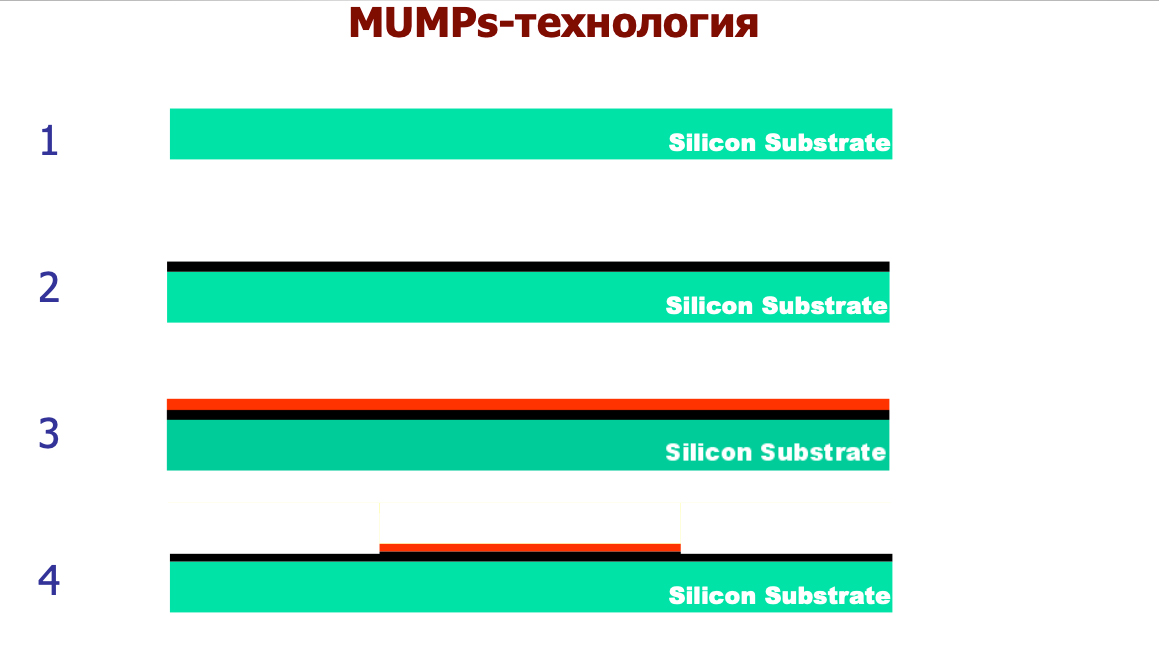
\includegraphics[width=1\linewidth]{1.jpg}}\\ \large {$\longmapsto$} \\
\end{minipage}
\hfill
\begin{minipage}[h]{0.4\linewidth}
\center{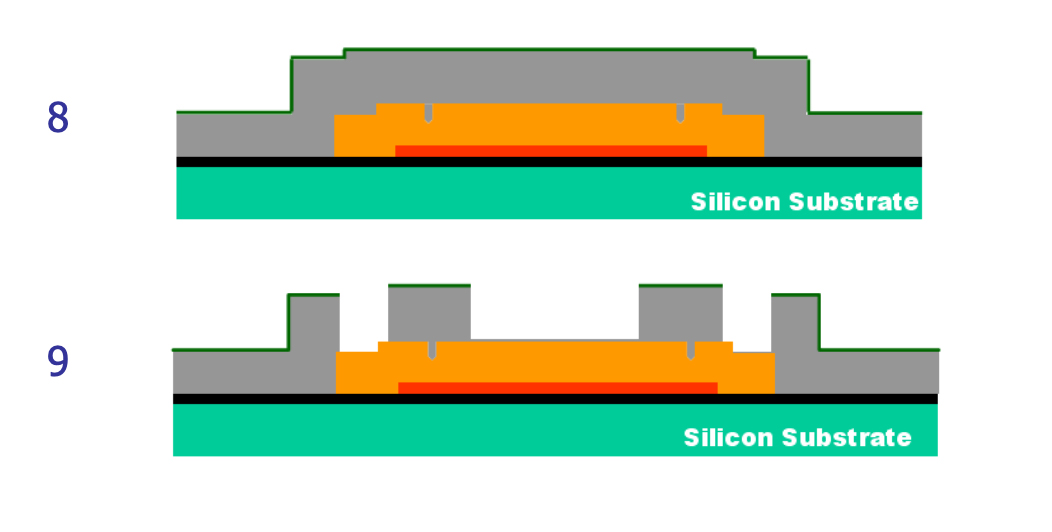
\includegraphics[width=1\linewidth]{22.jpg}} \huge{\textdownarrow} \\ 
\end{minipage}
\vfill
\begin{minipage}[h]{0.4\linewidth}
\center{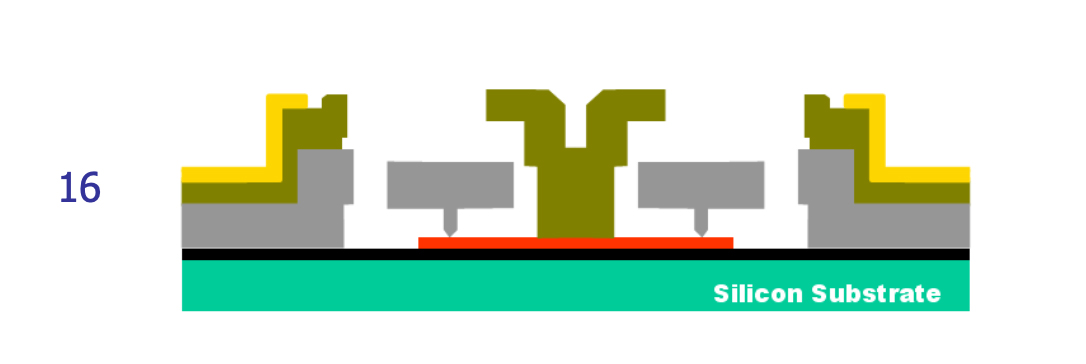
\includegraphics[width=1\linewidth]{5.jpg}}  $\bigstar$\\
\end{minipage}
\hfill
\begin{minipage}[h]{0.4\linewidth}
\center{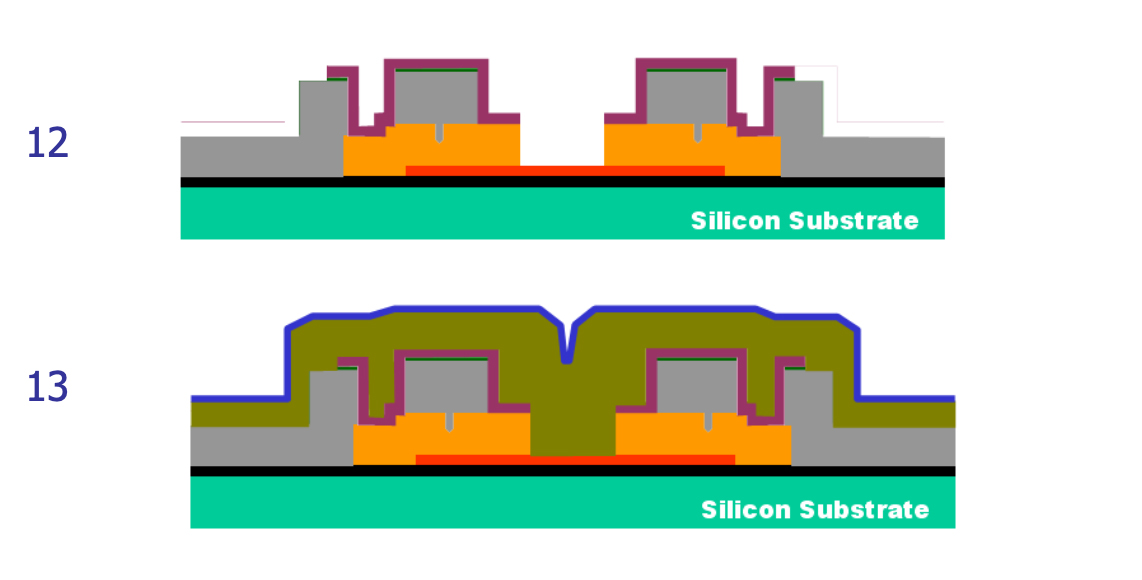
\includegraphics[width=1\linewidth]{4.jpg}} \Huge\textleftarrow\\
\end{minipage}
\label{ris:experimentalcorrelationsignals}
\end{figure}
\end{frame}
}



{
\title{\textcolor{orange}{Види елементів нанотехнологій}}
\usebackgroundtemplate{ 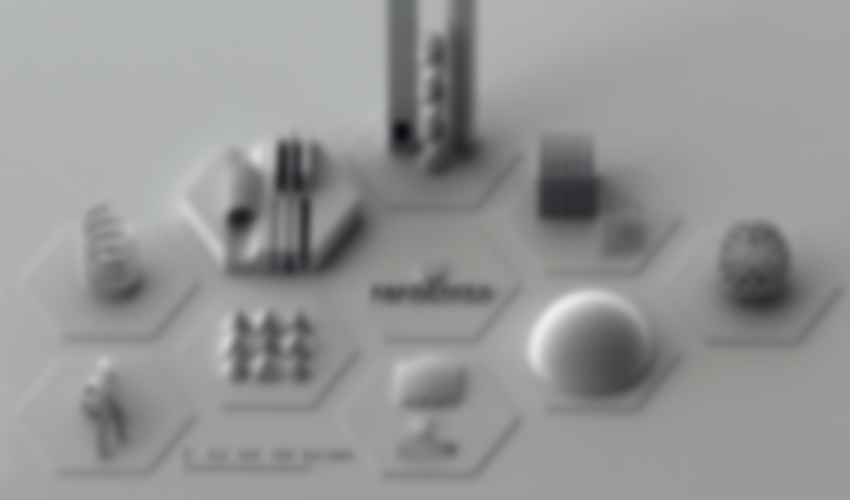
\includegraphics[width=\paperwidth,height=8.7cm]{nanoprint.jpg} }

\begin{frame}
\textcolor{black}{\fcolorbox{black}{yellow}{\large Також існують такі види елементів нанотехнологій:}}\\
\textbf{Атомна інженерія наноструктур.} Нанотехнологічні можливості скануючої
тунельної мікроскопії можна використовувати для керованої локальної модифікації поверхні з атомарною роздільною здатністю.\\
\textbf{Наноліторгафія.} Зменшення довжини світлової хвилі, використання Х- променів та електронного променя дозволяє створювати літографічні рисунки з розмірами елементів менше 100 нм.\\
\textbf{Напрофілювання.} Суть цього перспективного процесу створення
наноструктур полягає в тому, що оксидні плівки $\rm SiO_2$ товщиною менше 1нм
опромінюються гостро сфокусованим електронним променем при кімнатній
температурі. Оксид в опромінених ділянках розкладається і випаровується при
подальшій термообробці у вакуумі при температурі 720-7500°С.\\
\textbf{Нанодрук.} Використовуються два методи: класичний чорнильний друк
рисунків та механічне притискання штампу, поверхня якого покривається фарбою. Ці методи позбавлені таких недоліків як \textcolor{red}{дифракція} та \textcolor{red}{розсіяння хвиль}.
\end{frame}
}



{

\begin{frame}
\large\textcolor{blue}{\textbf {Питання№2}}\\
\textbf {Запишіть рівняння Гагена-Пуазейля для розподілу швидкості по радіусу труби, об’ємних та масових витрат рідини або газу. Сформулюйте поняття про приповерхневі температурні прошарки. Зробіть ескіз накладання поля швидкостей на поле приповерхневих температур для мікромеханічного перетворювача в потокоформуючому каналі.}
\end{frame}
}



{
\title{\textcolor{orange}{рівняння Гагена-Пуазейля}}
\usebackgroundtemplate{ 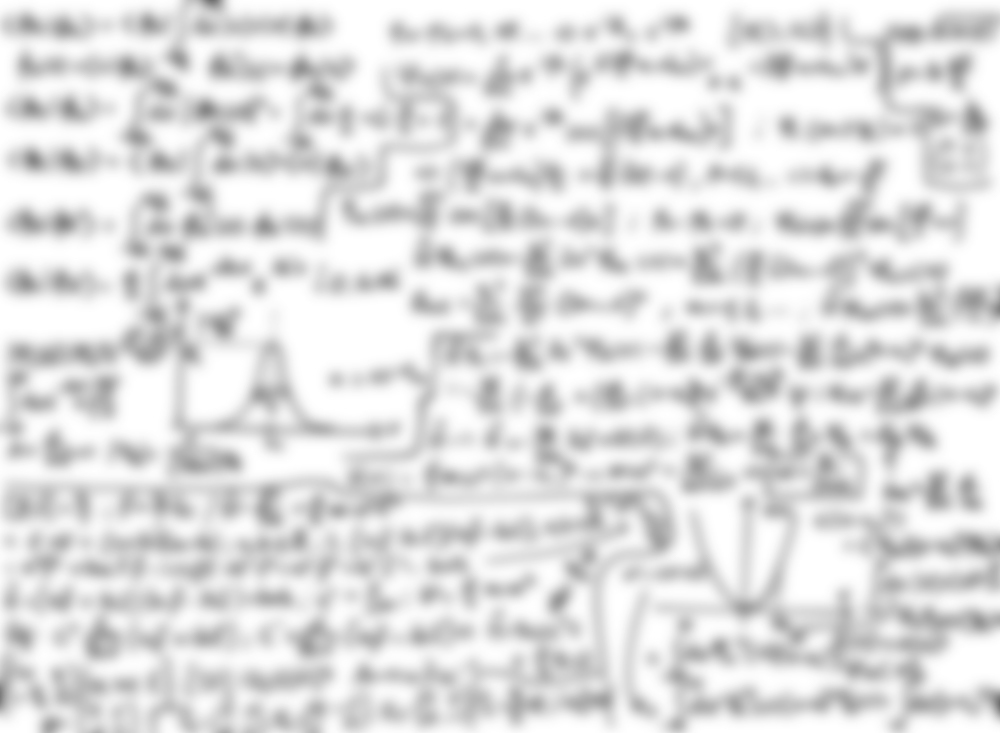
\includegraphics[width=\paperwidth]{formula.jpg} }
\begin{frame}
\textbf{Закон Пуазейля} — фізичний закон, що встановлює для ламінарної течії зв'язок між середньою швидкістю протікання рідини (або витратою) через капіляр та в'язкістю флюїду у залежності від перепаду тиску:
\[Q=\frac{\pi R^4 }{8\eta} \frac{\Delta p}L\]
де Q — об'єм флюїду, що протікає в одиницю часу (об'ємна витрата) через капіляр радіусом R та довжиною L при різниці тисків на кінцях капіляра $\rm\Delta p=p_{1}-p_{2},$
$\rm\eta$— коефіцієнт динамічної в'язкості.\\
\center\ {\textcolor{black}{\fcolorbox{black}{yellow}{\large Формулюється наступним чином:}}}\\
Об'ємна витрата рідини, що протікає прямолінійною ділянкою труби з круглим перетином сталого діаметра є прямо пропорційною перепаду тиску і четвертому степеню діаметра (радіуса) труби і обернено пропорційною її довжині.
\end{frame}
}



{
\title{\textcolor{orange}{Отримання закону Гагена-Пуазейля}}
\usebackgroundtemplate{ 
\includegraphics[width=\paperwidth]{idea.jpg} }
\begin{frame}
\textbf{\underline{Отримання закону:}}\\
Рівняння закону Пуазейля можна отримати шляхом інтегрування по площі перерізу рівняння розподілу швидкості в залежності від радіуса для круглоциліндричної труби:
{
\center ${\displaystyle Q=\int \limits _{S}v\left(r\right)dS=2\pi \int \limits _{0}^{R}v\left(r\right)rdr={\frac {\pi D^{4}(p_{1}-p_{2})}{128\eta L}}={\frac {\pi R^{4}(p_{1}-p_{2})}{8\eta L}},}$\\
}
де\\
Q — витрата рідини у трубопроводі;\\
D — діаметр трубопроводу.
\end{frame}
}



{
\title{\textcolor{orange}{Приповерхневі температурні прошарки}}
\usebackgroundtemplate{ 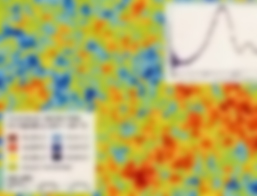
\includegraphics[width=\paperwidth]{x.jpg} }
\begin{frame}
Для аналізу процесів теплообміну традиційно використовується модель протікання ламінарного необмеженого потоку над плоскою поверхнею ізотермічного поверхневого тге, вбу- дованого врівень зі стінкою потоко-формуючого каналу. В середовищі формуються гідродинамічний і тепловий приповерхневі прошарки. Товщинa $\rm \delta_{v}(y)$ приповерхневого гідродина- мічного прошарку швидкості як функція коорди- нати вздовж потоку і теплофізичних параметрів рухомого середовища для потоку, необмеженого по нормалі до поверхні, визначається виразом:\\
\begin{center}
\small{$\displaystyle \rm \delta_{V}(y)=4,64\sqrt{\frac{\etaup_{FI}\cdotp y}		{\gammaup_{FI}\cdotp V_{\infty}}},$}\\
\end{center}
{
де y – координата вздовж напрямку руху потоку, відрахована від краю поверхні обтікання, {$\displaystyle\rm V_{\infty}$} - лінійна швидкість потоку на значному віддаленні від поверхні. 
}
Товщину приповерхневого прошарку температури в рухомому середовищі над нагрівачем знаходимо за виразом:\\
\begin{center}
\normalsize{$\displaystyle\rm \delta_{T}(y)=Pr^{-\frac{1}{3}}\cdotp \delta_{v}(y) = 4,68\sqrt{   \frac{\etaup_{fl}\cdotp (y-y_{0})}     {\gammaup_{FI}\cdotp V_{\infty}} } \cdotp Pr^{-\frac{1}{3}}  = 
4,68\sqrt{   \frac{\nuup_{fl}\cdotp (y-y_{0})}     {\gammaup_{FI}\cdotp V_{\infty}} } \cdotp Pr^{-\frac{1}{3}}  $},\\
\end{center}
де ${\rm(y-y_{0})}$ – координата вздовж напрямку руху потоку, відрахована від краю поверхні нагрівання, Pr – критерій прандтля.
\end{frame}
}



{
\usebackgroundtemplate{ 
\includegraphics[width=\paperwidth]{hh.jpg} }
\title{\textcolor{orange}{Приповерхневі температурні прошарки}}
\begin{frame}
\begin{figure}[h]
\begin{center}
 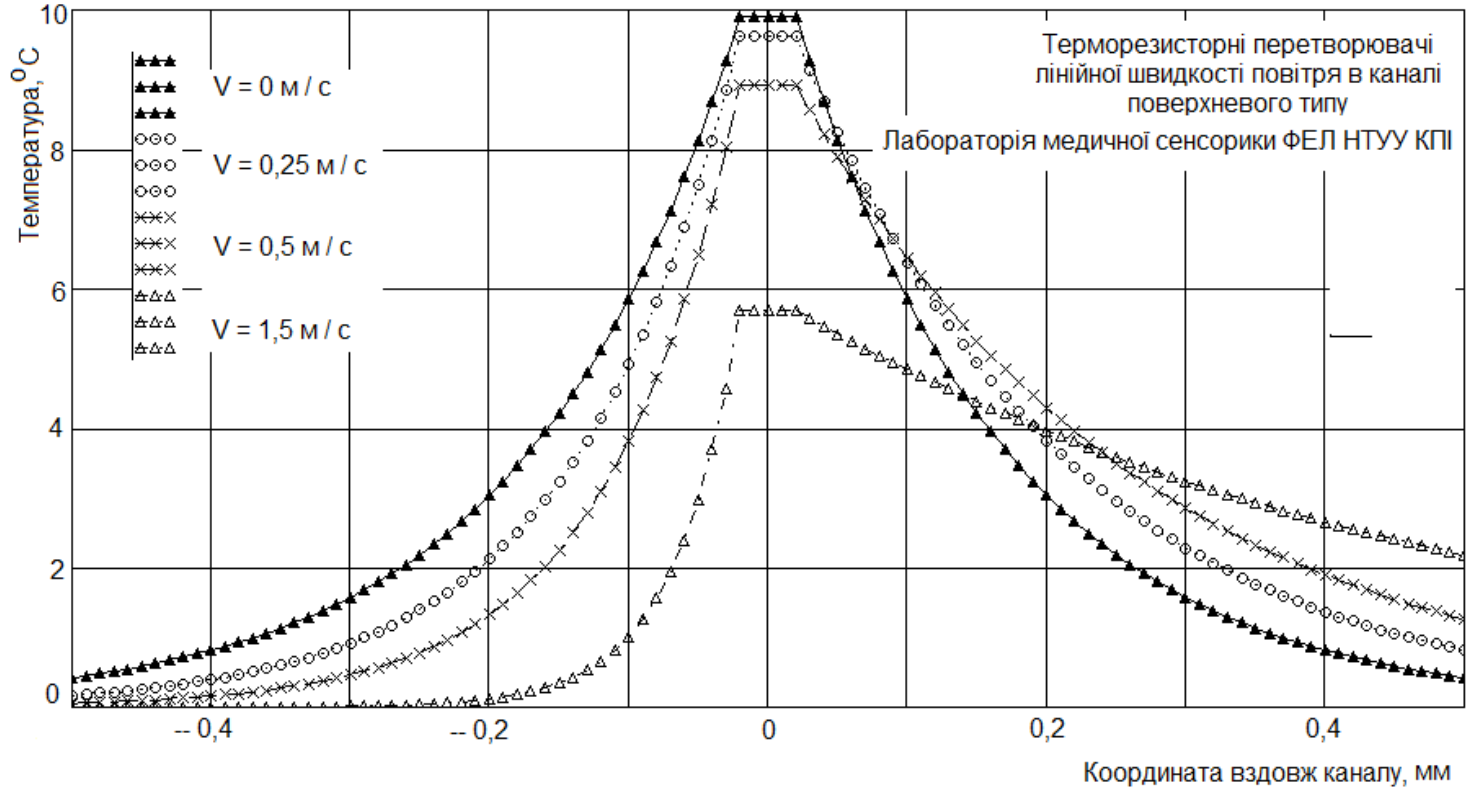
\includegraphics[scale=0.4]{g.png} 
\caption{Розрахункова залежність розподілу температури вздовж мембранного перетворювача від шви- дкості повітря в каналі висотою 300 мкм. Перетворювач поверхневого типу вмонтовано в стінку пото- коформуючого каналу. Товщина мембрани 0,4 мкм. Розміри термогенеруючого елементу 1000мкм х 40 мкм. Режим сталої потужності нагрівача Р=1 мВт}
\end{center}
\end{figure}
\end{frame}
 }



{

\begin{frame}
\large\textcolor{blue}{\textbf{Питання №3}}\\
\textbf {Наведіть схему інструментального (вимірювального) підсилювача на основі трьох ОП. Запишіть вираз для коефіцієнта перетворення.}
\end{frame}
}



{
\title{\textcolor{orange}{Інструментальний підсилювач для ОП}}
\usebackgroundtemplate{ 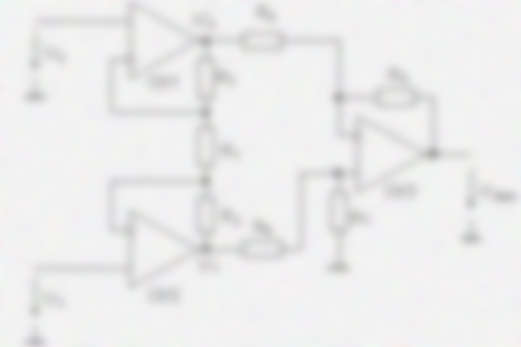
\includegraphics[width=\paperwidth]{3op.jpg} }
\begin{frame}
\textbf{Простий диференціальний підсилювач на одному ОП, має малий вхідний опір інвертувального входу. Низький вхідний опір, припустимий при використанні ДП з низькоомними джерелами сигналів, наприклад з тензометричним мостом. Однак він непридатний для роботи з високоомними джерелами.\\
Удосконалений ДП називають \underline{інструментальним} (або вимірювальним) підсилювачем (ІП). Такий підсилювач має високі й однакові опори на обох входах, установлення його коефіцієнта підсилення з високою точністю здійснюється за допомогою лише одного резистора, він має дуже високе пригнічення синфазного сигналу. ІП іноді називають потенціометричним підсилювачем, тому що він застосовується в пристроях перетворення потенціалів, що надходять як від заземлених, так і від незаземлених джерел сигналів.}
\end{frame}
}









{
\title{\textcolor{orange}{Інструментальний підсилювач}}
\usebackgroundtemplate{ 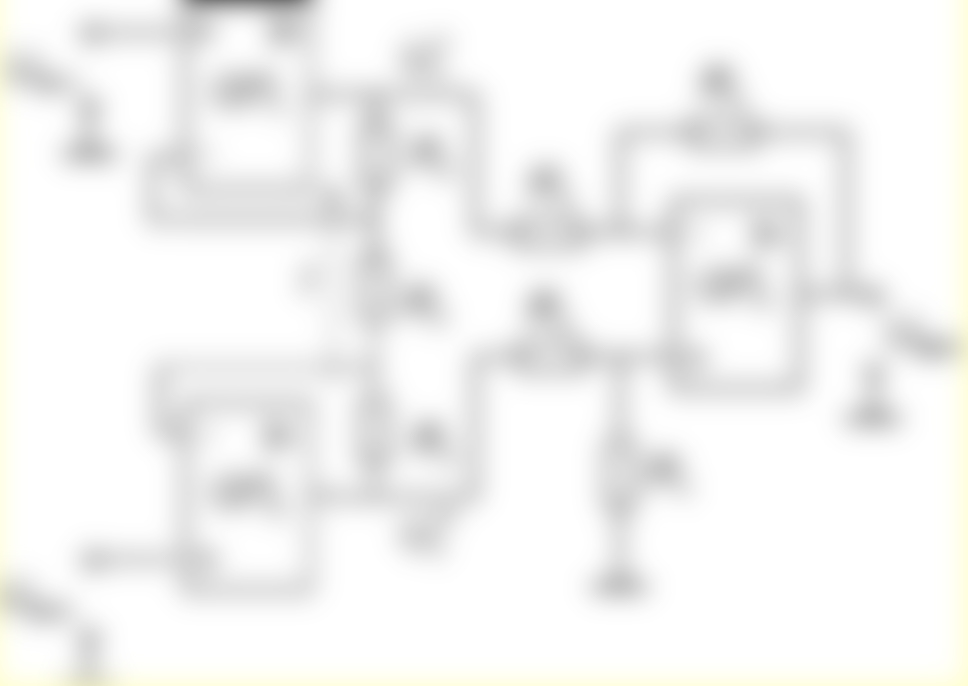
\includegraphics[width=\paperwidth]{op.jpg} }
\begin{frame}{Інструментальний підсилювач з потенціометром}

\begin{figure}[!ht]
\begin{center}
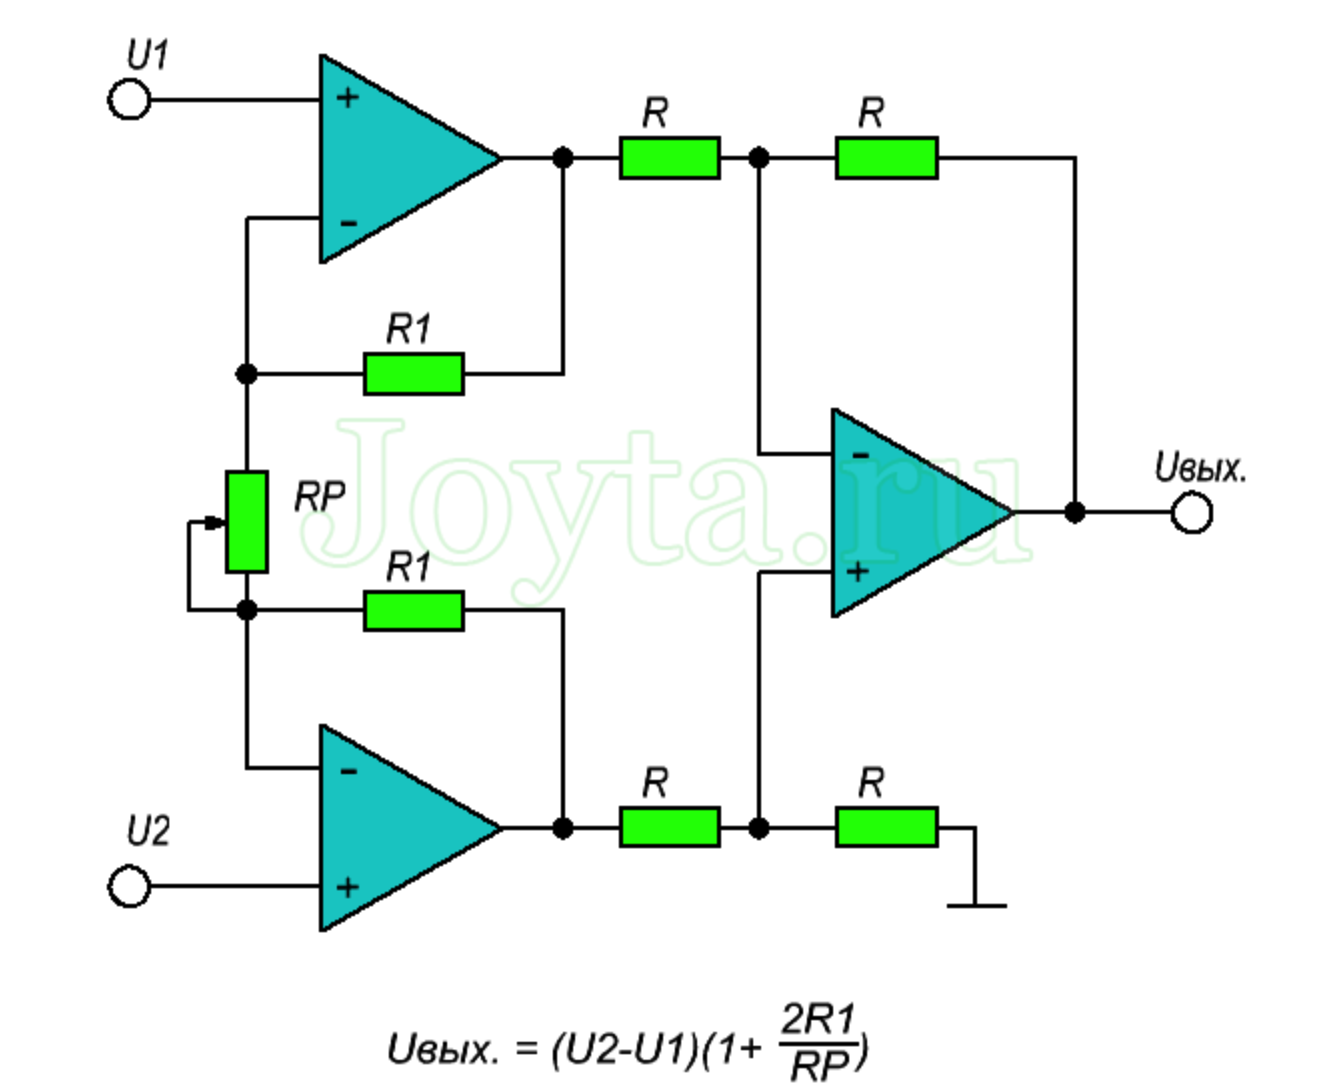
\includegraphics[scale=0.33]{bbb.png}
\caption{Інструментальний підсилювач для трьох ОП}
\end{center}
\end{figure}
\end{frame}
}








{
\title{\textcolor{orange}{Інструментальний підсилювач}}
\usebackgroundtemplate{ 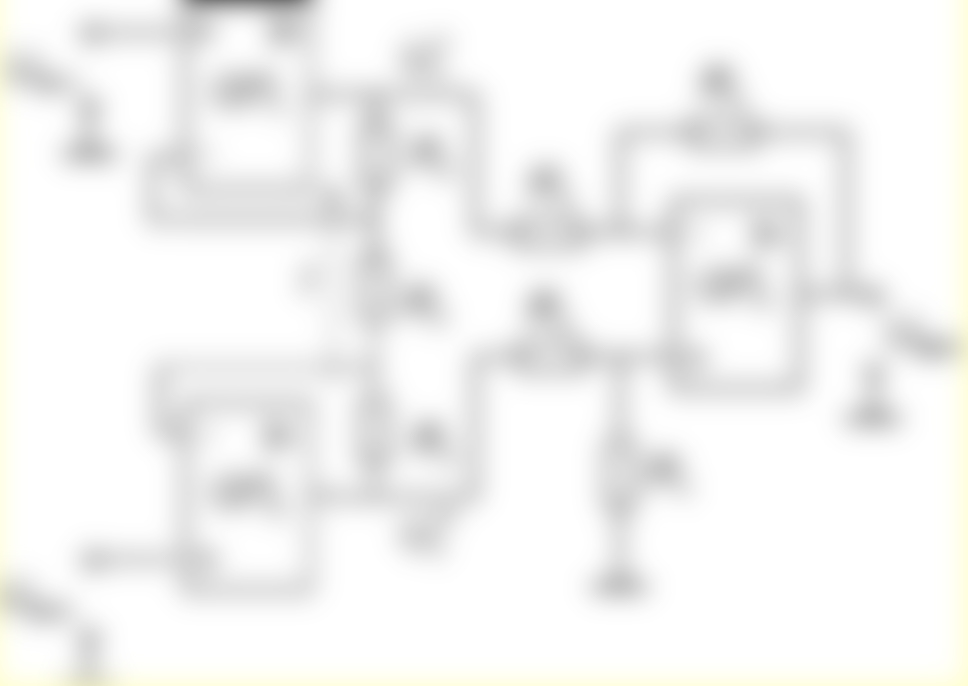
\includegraphics[width=\paperwidth]{op.jpg} }
\begin{frame}
\textbf {Коефіцієнт посилення синфазного сигналу (через розбаланс резисторів):}\\
\center{$\displaystyle \rm K= \frac{R_{7}R_{4} -R_{5}R_{6}} 
		     				   {R_{4}(R_{6}+R_{7})}$ }
\begin{figure}[!ht]
\begin{center}
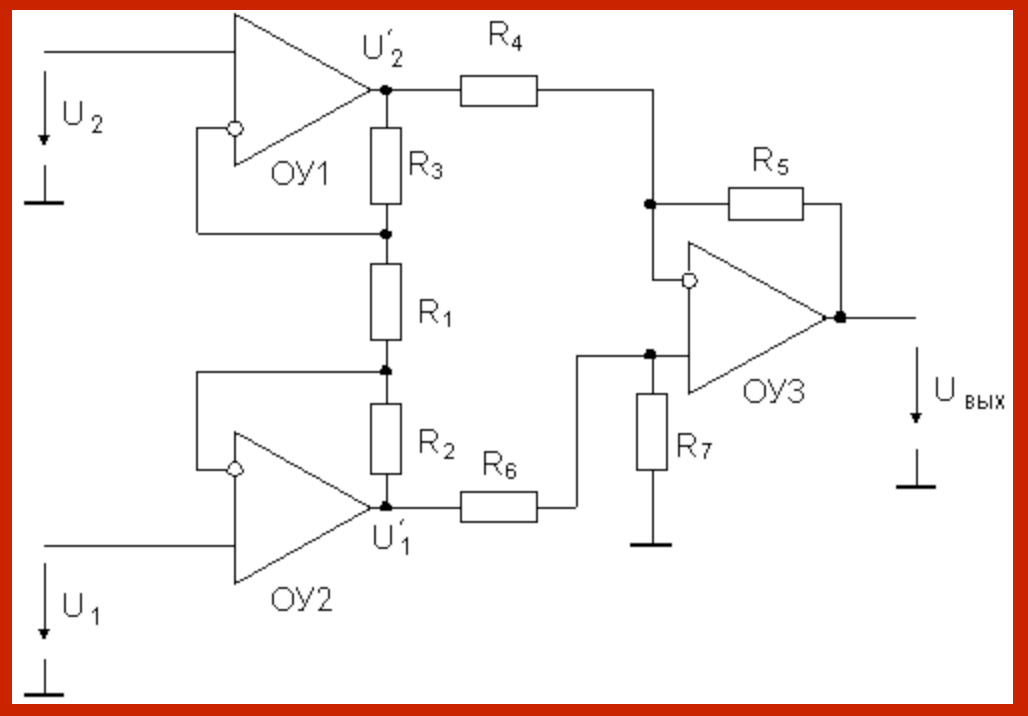
\includegraphics[scale=0.2]{33op.jpg}
\caption{Інструментальний підсилювач для трьох ОП}
\end{center}
\end{figure}
\end{frame}
}






{



\begin{frame}% второй слайд
\textcolor{blue}{\large Доп. Питання}\\
%\textbf{\textit{(Bold italic) Жирный курсив}}\\
\Large{Назвіть області, на Ваш погляд, найбільш ефективного застосування сучасних мікроелектромеханічних систем (МЕМС) або \underline{приклади}, на Ваш погляд, найбільш вдалих і перспективних комерційно доступних МЕМС у масовому виробництві.}
\end{frame}
}



{
\title{\textcolor{orange}{Доп. Питання}}
\usebackgroundtemplate{ 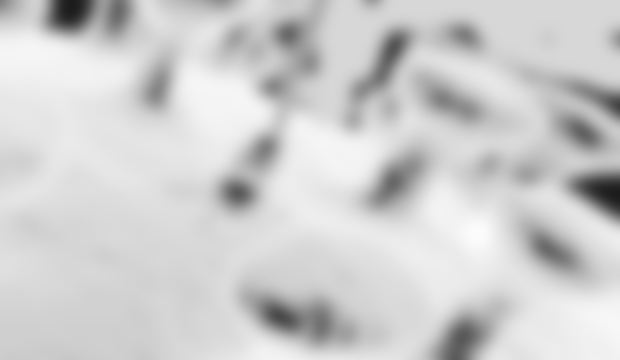
\includegraphics[width=\paperwidth]{nan.jpg} }
\begin{frame}
\center{\fcolorbox{black}{orange}{\href{https://habr.com/ru/post/7202/}{\underline {Smart Dust}-ссылка на хабр}}}\\
\begin{minipage}[h]{0.3\linewidth}
\center{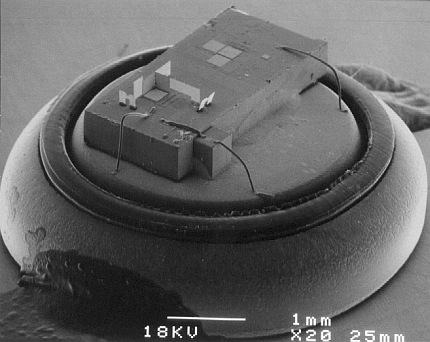
\includegraphics[width=1.2\linewidth]{nano.jpg}} Приклад №1\\ 
\end{minipage}
\hfill
\begin{minipage}[h]{0.38\linewidth}
\begin{center}
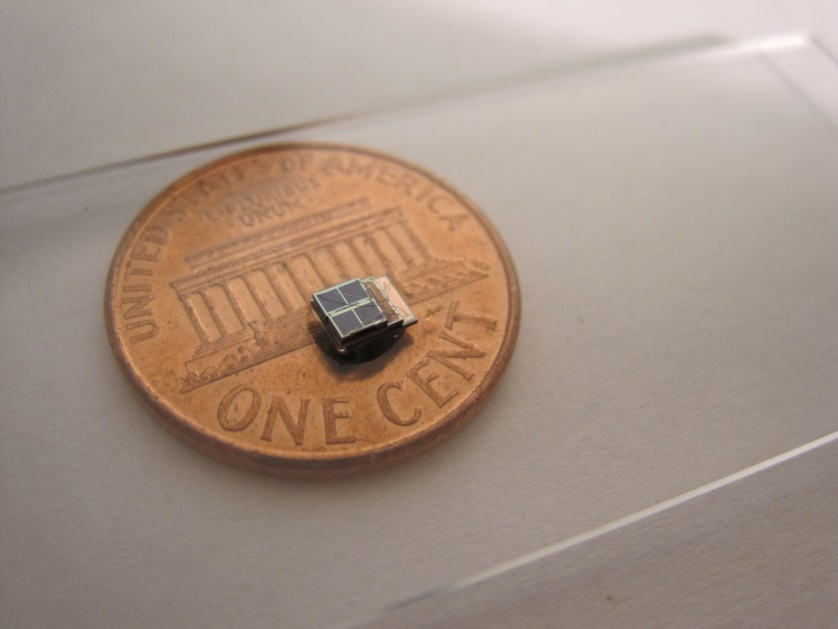
\includegraphics[width=1\linewidth]{nano1.png} \\ Приклад №2
\end{center}
\end{minipage}\\
\small Найбільш очевидне і просте у виконанні завдання, яке можна буде доручити вже найпершим, порівняно великим, стайним нанороботам - фізичне знищення сил противника за допомогою мікрозарядів вибухівки. Будучи скинутими з літака (авжеж, безпілотного) хмара самеа автоматично шукає ціль, розділяється на кластери необхідного для їх ураження розміру, обліплює їх, проникаючи в незахищені місця, і синхронно підривається. Одержаний \\ об'ємний вибух спалює системи управління технікою і спустошує найзахищеніші бомбосховища з максимальною ефективністю, недоступною звичайним видам озброєння.
\end{frame}
}



{
\title{\textcolor{orange}{Smart Dust}}
\usebackgroundtemplate{ 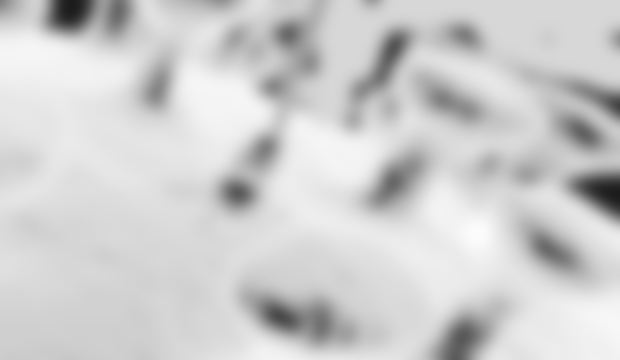
\includegraphics[width=\paperwidth]{nan.jpg} }
\begin{frame}
%\center{\fcolorbox{black}{orange}{\href{http://fkn.ktu10.com/?q=node/2906}{\underline {Smart Dust}-ссылка}}}\\

\center{
\begin{minipage}[h]{0.4\linewidth}

{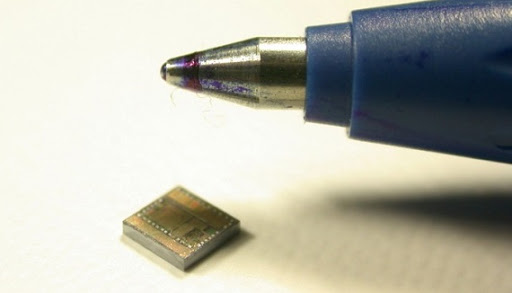
\includegraphics[width=0.79\linewidth]{111.jpg}} \small  \center{ Приклад №3}\\ 

\end{minipage}\\
}
%\hfill
%\begin{minipage}[h]{0.38\linewidth}
%\center{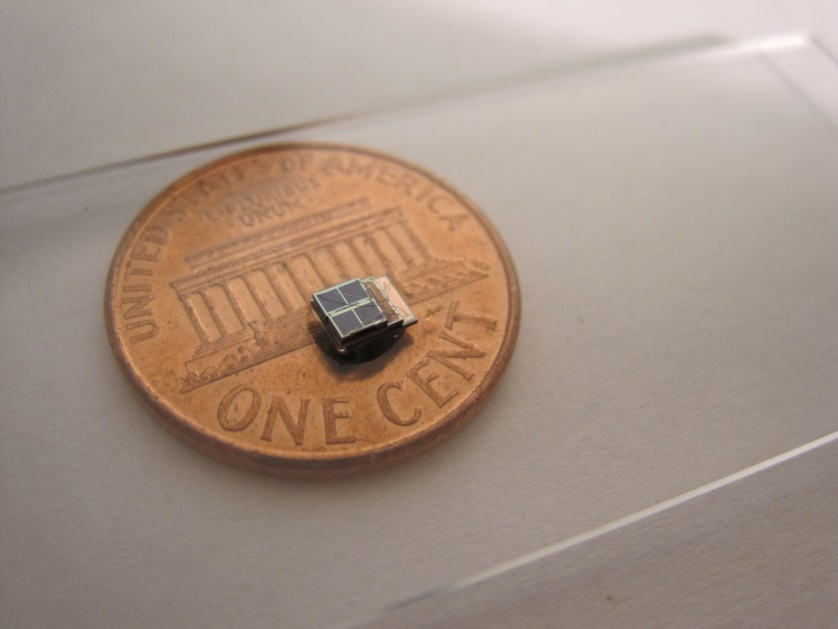
\includegraphics[width=1\linewidth]{nano1.png}} \\ Приклад №2
%\end{minipage}\\
\small
Також як наприклад, більш мирного застосування: розвідка місцевості та шпигунство; ця задача вимагає набагато складніших програмних алгоритмів і можливості використання складних засобів спостереження і зв'язку. Тому, за прогнозами фахівців, воно стане здійсненно за допомогою розумного пилу не раніше, ніж через 7-10 років (інформація взята зі статті 2007 року). Сценарій дій тут буде наступним. Розпорошена в околицях важливого об'єкта хмара непомітно переміщається в його сторону, попутно вибираючи оптимальні місця для розміщення спеціалізованих субоблачков. Хмара відеоспостереження, кожна порошинка якого є окремий піксель матриці з інтерфейсом зв'язку з сусідами, прагне зайняти кращу позицію для більшого огляду простору. Жучки (або, можливо, «мошки») встановлюють контроль за звуками. Найскладніша частина, передача інформації в штаб розвідки, найближчим часом навряд чи зможе обійтися без засилання агента з пристроєм, що зчитує її як в сучасних RFID-системах.
\end{frame}
}









\end{document}